\documentclass[
  11pt,
  letterpaper,
   addpoints,
   answers
  ]{exam}

\usepackage{../exercise-preamble}
\usepackage{wrapfig}
\usepackage{subfigure}
\usepackage{float}
\begin{document}

\noindent
\begin{minipage}{0.47\textwidth}

\includegraphics[width=\textwidth]{../fcfm_die}
\end{minipage}
\begin{minipage}{0.53\textwidth}
\begin{center} 
\large\textbf{Conversión de la Energía y Sistemas Eléctricos } (EL4111-1) \\
\large\textbf{Resumen Control 2} \\
\small Prof.~Constanza Ahumada - Rodrigo Moreno.\\
\small Prof.~Aux.~Javiera Pacheco - Erik Sáez\\
\small Ayudantes.~Manuel Aceituno - Pamela Acuña - Alvaro Flores\\
\end{center}
\end{minipage}

\vspace{0.5cm}
\noindent
\vspace{.85cm}
\hrule

\section*{Maquina de Corriente Continua}
\subsection*{Aspectos constructivos}
\begin{minipage}{0.6\textwidth} % Parte izquierda con el texto
  \begin{itemize}
      \item Un sistema colector el cual está formado por delgas y escobillas, produce que el voltaje de salida de una máquina CC se encuentre rectificado, al aumentar la cantidad de delgas el voltaje de salida se rectifica aún más. Estas están hechas de carbón, grafito o una mezcla, con una conductividad alta para reducir las pérdidas eléctricas y bajo coeficiente de fricción para reducir el desgaste.
      \item El voltaje de salida de una máquina CC debido a la relación no lineal entre la corriente de excitación $i_{c}$ y el campo magnético, no será una sinusoide perfecta.
      \item Existen dos devanados, siendo el primero el de armadura que es donde se induce el voltaje y se ubica en el rotor y el segundo es el de campo que se ubica en el estator, que son los responsables de generar el flujo magnético.
      \item Existen dos tipos de construcciones para los polos, achaflanada o excéntrica. Siendo la última con una forma más curva lo que permite distribuir mejor el flujo magnético de manera más uniforme.
      \item El conmutador se construye sobre el eje del rotor, y se encarga de invertir la polaridad de la corriente en la armadura, y está hecho sobre barras de cobre aisladas entre sí.
  \end{itemize}
\end{minipage}%
\hfill
\begin{minipage}{0.35\textwidth} 
  \centering
  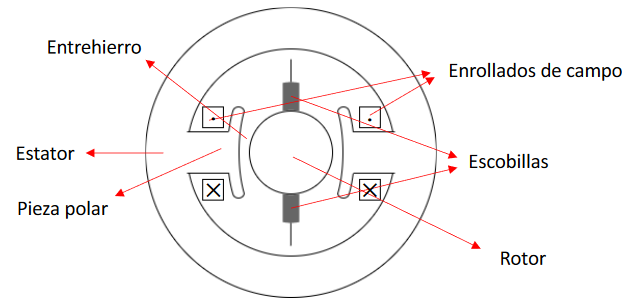
\includegraphics[width=\linewidth]{Resumen_1} 
  \captionof{figure}{Diagrama del motor de corriente continua.}
\end{minipage}
\subsection*{Modelo circuital}
\begin{minipage}{0.6\textwidth}
    \begin{align*}
        V_c &= L_c \frac{di_c}{dt} + R_c i_c \\
        V_a &= E_a \pm L_a \frac{di_a}{dt} \pm R_a i_a \\
        T_{\text{ind}} &= \frac{E_a i_a}{\omega} \\
        J \frac{d\omega}{dt} &= T_{\text{mec}} \pm T_{\text{ind}}
    \end{align*}
\end{minipage}%
\hfill
\begin{minipage}{0.45\textwidth} 
    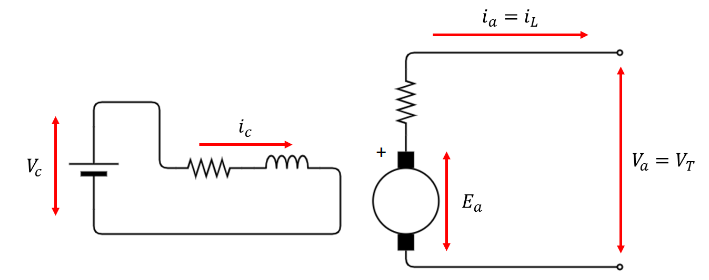
\includegraphics[width=1\linewidth]{Resumen_2} 
    \captionof{figure}{Modelo circuital para una maquina CC general.}
\end{minipage}
\begin{itemize}
  \item $V_c, i_c$ son la tensión aplicada y la corriente entrando al circuito de campo.
  \item $V_a, i_a$ son la tensión aplicada y la corriente entrando a la armadura.
  \item $E_a$ es la fem generada en la armadura.
  \item $T_{\text{ind}}$ es el torque electromagnético inducido en el rotor y $\omega$ es la velocidad de giro del rotor.
  \item $J$ es el momento de inercia del rotor y las masas acopladas al eje.
  \item $R_c, R_a, L_c$ y $L_a$ son las resistencias e inductancias de campo y de armadura.
\end{itemize}
Ademas se tiene que para un solo campo:
\begin{align}
  E_a &= K \phi \omega = G \omega i_{c}\\\
  T_{\text{ind}} &= G i_{c}i_{a}
\end{align}
Donde k coresponde a una constante de diseño y G se denomina inductancia de rotacion, estos parametros no son constantes, pero se pueden considerar dentro de pequeños rangos de operacion.
\begin{itemize}
  \item \textbf{Perdidas en el nucleo:} Producto de la histeriris y corrientes parasitas, las cuales aumentan con la densidad de flujo magnetico y la velocidad de operacion:
  \item \textbf{Perdidas mecanicas:} Debido a la friccion y el rozamiento con el aire, estas aumentan con la velocidad de operacion.
  \item \textbf{Perdidas en el cobre:} Se presentan en los devanados de campo y armadura de la maquina.
  \begin{align}
    P_a &= i_a^2 R_a \quad \text{(Pérdidas en la armadura)} \\
    P_c &= i_c^2 R_c \quad \text{(Pérdidas en el campo)}
  \end{align}
  Donde $R_{a}$ y $R_{c}$ son las resistencias de armadura y campo respectivamente.
  \item \textbf{Perdidas por caida de tension en las escobillas}: Se produce debido al contacto entre las escobillas y el conmutador, estas aumentan con la corriente de armadura.
\end{itemize}

  \begin{align}
    P_{Ce} = \Delta V_{Ce} i_{a}
  \end{align}
  Donde $\Delta V_{Ce}$ es la caida de tension en las escobillas. Es posible el pasar de una configuracion de maquina CC de excitacion independiente a dos modelos circuitales equivalentes, dados por:
  \begin{figure}[H]
    \begin{center}
      \subfigure[Maquina CC de excitacion en serie]{
          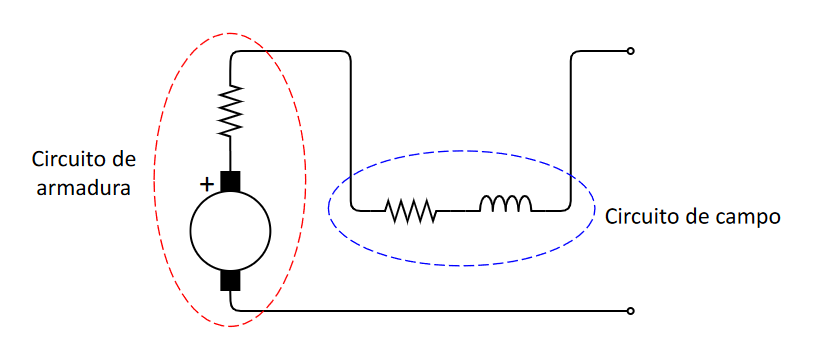
\includegraphics[width=0.35\textwidth]{Resumen_3}
          \label{Imagen-Madrid}}
      \subfigure[Maquina CC de excitacion en Paralelo]{
          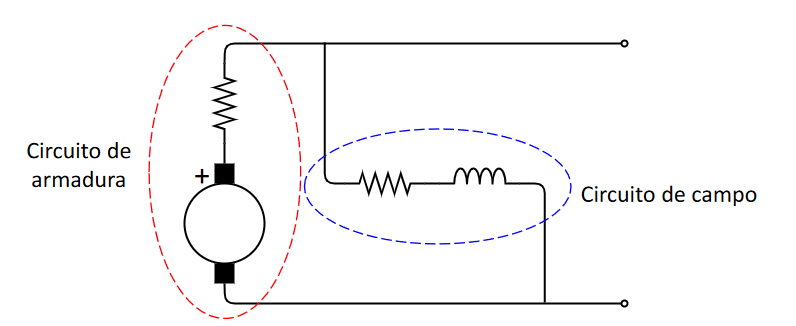
\includegraphics[width=0.35\textwidth]{Resumen_4}
          \label{Imagen-Paris}}
      \subfigure[Maquina CC compuesta]{
          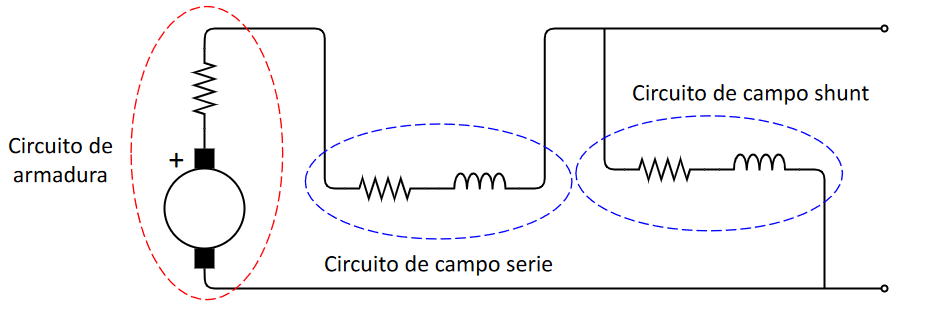
\includegraphics[width=0.35\textwidth]{Resumen_5}
          \label{Imagen-Londres}}
      \label{Figura-Ciudades}
    \end{center}
  \end{figure}  
Luego es posible caracterizar las eficiencia por:
\begin{align}
  &\text{La eficiencia de cualquier máquina eléctrica:} \quad \eta = \frac{P_{\text{out}}}{P_{\text{in}}} \\
  &\text{Eficiencia generador} \quad \eta = \frac{V_T i_L}{T_{\text{ap}}\omega} \\
  &\text{Eficiencia Motor} \quad \eta = \frac{T_{\text{ap}}\omega}{V_T i_L} \\
  &\text{La regulación de voltaje generador:} \quad Reg = \frac{V_0 - V_T}{V_T}
\end{align}
Donde $V_{0}$  es la tension en bornes en vacio
%------------------------------------------------------------------
\subsection*{Analisís en estado estacionario}
Para analizar el desempeño de una maquina CC cn cualquier tipo de conexion y operando como generador o motor, se tienen diversas curvas caracteristicas, algunas de estas son:
\begin{figure}[h!]
  \centering
  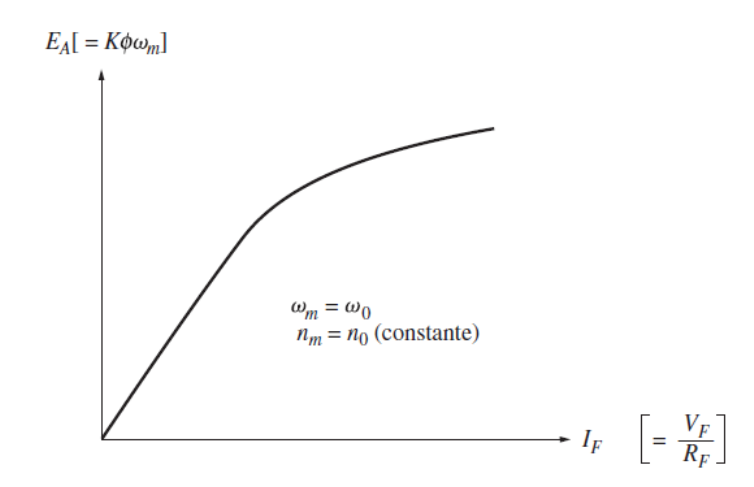
\includegraphics[width=0.5\textwidth]{Resumen_6}
  \caption{Ejemplo de una curva de maquina CC, en particular corresponde a una curva de magnetizacion, es interesante mencionar que tanto motores como generadores estan diseñados para operar cerca del punto de operacion , eso quiere decir que se requiere un gran incremento en la corriente de campo para un pequeño incremento en la tension de salida.}
\end{figure}
\begin{itemize}
  \item En el generador de excitación independiente el flujo de campo se deriva de una fuente de potencia separada e independiente del generador en sí mismo.
  \item En esta configuracion si se desea controlar el voltaje en las terminales se puede hacer de dos maneras
  \begin{itemize}
    \item Si se aumenta la velocidad de rotacion $\omega$ entonces aumenta la tension interna
    \item Si se aumenta la corriente de campo $i_{c}$ aumentara el flujo en la maquina y por lo tanto la tension interna (\textit{En la practica se utiliza este metodo dado que variar la velocidad de rotacion suele estar limitado})
  \end{itemize} 
\end{itemize}
Se tienen las diferentes configuraciones de conexion para una maquina CC, las cuales son:

\subsection*{Generador CC en Derivación}
\begin{minipage}{0.6\textwidth} % Parte izquierda con las ecuaciones
    \begin{align*}
        V_c &= R_c i_c \\
        V_a &= E_a - R_a i_a \\
        E_a &= G \omega i_c \\
        T_{\text{ind}} &= \frac{E_a i_a}{\omega} = G i_c i_a \\
        T_{\text{mec}} - T_{\text{ind}} &= 0 \\
        V_T &= V_a = V_c \\
        i_a &= i_c + i_L
    \end{align*}
\end{minipage}%
\hfill
\begin{minipage}{0.35\textwidth} % Parte derecha con la imagen
    \centering
    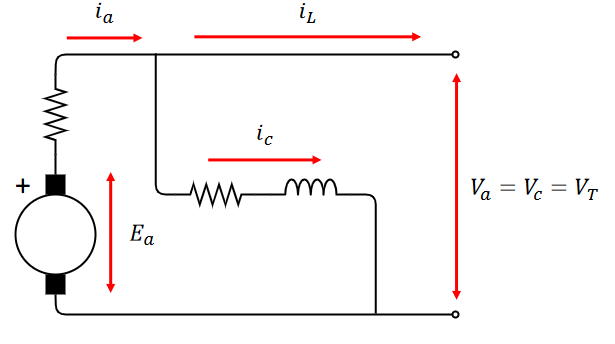
\includegraphics[width=1\linewidth]{Resumen_8} % Coloca la ruta correcta de tu imagen
    \captionof{figure}{Diagrama del generador CC en derivación.}
\end{minipage}
\vspace{1cm} 

\subsection*{Generador CC en Serie}
\begin{minipage}{0.6\textwidth} % Parte izquierda con las ecuaciones
    \begin{align*}
        V_c &= R_c i_c \\
        V_a &= E_a - R_a i_a \\
        E_a &= G \omega i_c \\
        T_{\text{ind}} &= \frac{E_a i_a}{\omega} = G i_c i_a \\
        T_{\text{mec}} - T_{\text{ind}} &= 0 \\
        V_a &= V_c + V_T \\
        i_a &= i_c = i_L
    \end{align*}
\end{minipage}%
\hfill
\begin{minipage}{0.35\textwidth} % Parte derecha con la imagen
    \centering
    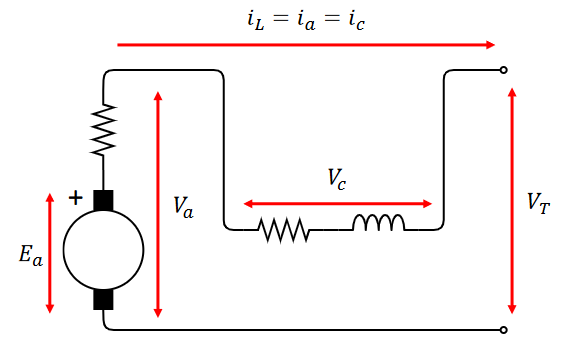
\includegraphics[width=1\linewidth]{Resumen_9} % Coloca la ruta correcta de tu imagen
    \captionof{figure}{Diagrama del generador CC en serie.}
\end{minipage}
\vspace{1cm} 

\subsection*{Motor CC en derivacion}
\begin{minipage}{0.6\textwidth} % Parte izquierda con las ecuaciones
    \begin{align*}
        V_c &= R_c i_c \\
        V_a &= E_a + R_a i_a \\
        E_a &= G \omega i_c \\
        T_{\text{ind}} &= \frac{E_a i_a}{\omega} = G i_c i_a \\
        T_{\text{mec}} - T_{\text{ind}} &= 0 \\
        V_T &= V_a = V_c \\
        i_L &= i_a + i_c
    \end{align*}
\end{minipage}%
\hfill
\begin{minipage}{0.35\textwidth} % Parte derecha con la imagen
    \centering
    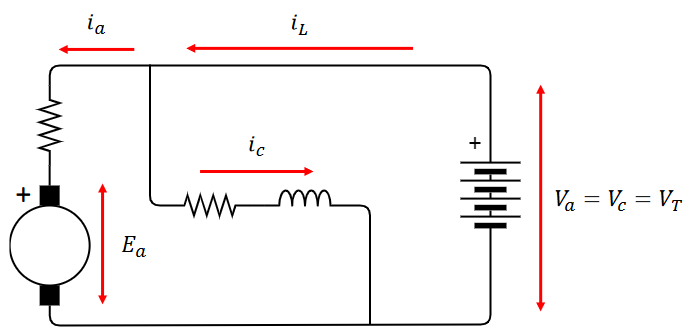
\includegraphics[width=1.1\linewidth]{Resumen_10} % Coloca la ruta correcta de tu imagen
    \captionof{figure}{Diagrama del motor CC en serie}
\end{minipage}
\subsection*{Motor CC en serie}
\begin{minipage}{0.6\textwidth} % Parte izquierda con las ecuaciones
  \begin{align*}
      V_a &= V_c + V_T \\
      i_a &= i_c = i_L \\
      V_c &= R_c i_L \\
      V_a &= E_a - R_a i_L \\
      E_a &= G \omega i_L \\
      T_{\text{ind}} &= \frac{E_a i_L}{\omega} = G i_L^2 \\
      T_{\text{mec}} - T_{\text{ind}} &= 0
  \end{align*}
\end{minipage}%
\hfill
\begin{minipage}{0.35\textwidth}
  \centering
  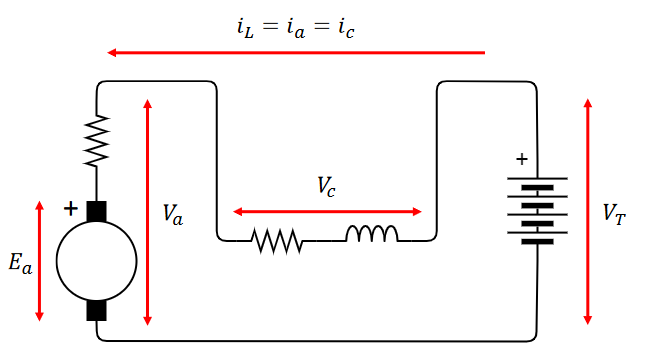
\includegraphics[width=1\linewidth]{Resumen_11} 
  \captionof{figure}{Motor CC en serie}
\end{minipage}\\\\
Para controlar la velocidad de un motor CC en derivacion existen dos metodos:
\begin{itemize}
  \item Ajustando la resistencia del circuito de campo , mediante una ressitencia variable.
  \item Modificando la tension en las terminales aplicadas a los bornes de la maquina
\end{itemize}
\subsection*{Reaccion de armadura}
Si se conecta una carga a los bornes de las escobillas, flutye una corriente que circula por la carga y por los devanados de la armadura, este flujo de corriente produce un campo magnetico propio el cual distorsiona el campo magnetico original, este fenomeno se conoce como reaccion de armadura, lo cual produce dos fenomenos dados por: (\textit{Para entender de mejor manera este concepto recomiendo \href{https://www.youtube.com/watch?v=R0cyZ052zJ0&t=161s}{este video}}) 
\begin{itemize}
  \item Desplazamiento del plano magnetico neutro
  \item Debilitamiento del campo
\end{itemize}
Para el primer caso es importante destacar que en caso de operar como generador el plano neutro se desplaza en el sentido de la rotación. Si esta máquina hubiera sido un motor, la corriente de armadura fluye en dirección opuesta y el plano de desplaza contra el sentido de rotación.\\\\
El problema con el desplazamiento del plano neutro es que el conmutador debe provocar un cortocircuito en los segmentos de las delgas justo en el instante en que el voltaje a través de ellos es nulo. Este problema es grave puesto que lleva a que la vida útil de las escobillas se reduzca de manera drástica, y a que se deterioren las delgas\\\\
Por otro lado el debilitamiento del campo se produce debido a la curva de magnetizacion y al hecho de que algunas zonas de la superficie polar, el flujo magnético del rotor se suma al flujo del campo principal, lo que provoca un ligero aumento en el flujo total en esas áreas.Este problema se encuentra presentae tanto en generadores como en motores.  En general se tiene que cuando disminuye el flujo de un motor se incrementa su velocidad. Pero el incrementar la velocidad de un motor aumenta su carga, lo que provoca un debilitamiento aún mayor del flujo. 

\subsection*{Metodos de solucion}
Existen algunos metodos para corregir el problema de la reaccion de armadura, algunos de estos son:
\begin{itemize}
  \item \textbf{Desplazamiento de las escobillas:} El desplazamiento de las escobillas en un motor o generador se utiliza para alinearlas con el plano magnético neutro y reducir la generación de chispas, pero esta técnica presenta problemas: el plano neutro cambia con cada variación de carga y se invierte cuando la máquina cambia entre modos de motor y generador, lo que exige ajustes constantes. Además, aunque ayuda a controlar las chispas, este desplazamiento debilita el flujo magnético, afectando la eficiencia del equipo.
  \item \textbf{Polos de Conmutacion:} Se emplean polos de conmutación, ubicados entre los polos principales, que permiten reducir el voltaje en los conductores durante la conmutación, evitando chispas. Estos polos no afectan el flujo principal y sólo influyen en los conductores en el momento exacto de la conmutación. Al incrementarse la carga, el efecto del flujo de los interpolos se opone al desplazamiento del plano neutro, logrando una cancelación que mantiene el funcionamiento estable tanto en modo motor como generador.
  \item \textbf{Devanados de compensacion:} Los devanados de compensación se utilizan en motores de trabajo pesado para eliminar completamente la reacción de armadura y estabilizar el flujo de campo, evitando así el desplazamiento del plano neutro. Estos devanados se ubican en las caras de los polos y generan una fuerza magnetomotriz opuesta a la del rotor, neutralizando su efecto. Como resultado, el flujo en la máquina se mantiene constante independientemente de la carga, asegurando un rendimiento estable.
\end{itemize}
%-------------------------------
\newpage
\hrule
\section*{Ejemplos: Preguntas de contenido Maquinas CC}
\begin{questions}
  \question \textbf{Control Primavera 2023} Qué es la reacción de la armadura de la máquina de CC? Coment sus efectos en la generación eléctrica y soluciones propuestas
  \begin{solution}
    La reacción de armadura es el campo magnético inducido en la armadura de la máquina de corrien- te continua debido al movimiento del rotor. Este campo inducido distorsiona el flujo magnético provocando desplazamiento del campo magnético neutro y causa el debilitamiento del campo ori-
    ginal. Dentro de las posibles soluciones se encuentra: Desplazamiento de las escobillas, el uso de polos de conmutación y el uso de devanados de compensación
  \end{solution}
  \question \textbf{Control Otoño 2024} El motor de CC en conexión shunt no debe utilizarse sin carga mecánica, porque existe el riesgo de embalamiento
  \begin{solution}
    Falso. Al igual que en caso de la máquina de C.C. conectada como generador, existen curvas que per miten explicar el comportamiento de los motores y estimar su desempeño de acuerdo a las distintas configuraciones de conexión. En este sentido una de las curvas características de los motores de C.C. más representativa es la curva de Torque -velocidad, representada en la siguiente figura para la conexión shunt
    \begin{center}
      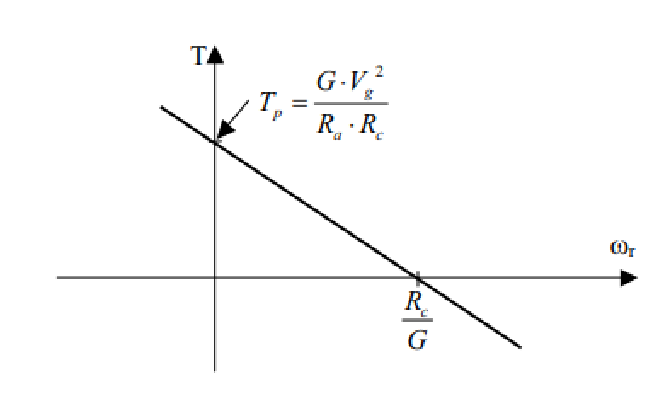
\includegraphics[width=0.4\textwidth]{Resumen_12} \\
      \textit{Curva Torque-velocidad de un motor shunt}
  \end{center} 
    Si la máquina está operando como motor y se aumenta la velocidad de giro, el torque generado comienza a disminuir hasta el punto en que se torna cero, si en este caso se sigue aumentando la velocidad entonces la corriente de armadura se invierte y la máquina comienza a operar como generador. Por ende, no ocurre el fenómeno de embalamiento, el cual si ocurre en los motores en serie
    \begin{center}
      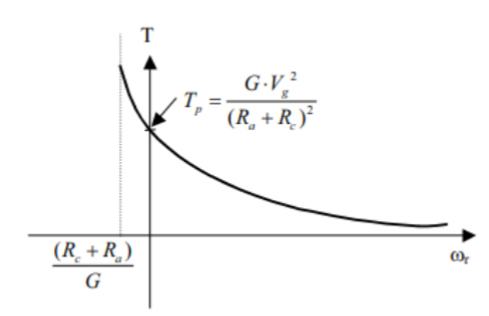
\includegraphics[width=0.4\textwidth]{Resumen_13} \\
      \textit{Curva Torque-velocidad de un motor en serie}
  \end{center}
    \end{solution}
    \question \textbf{Control Otoño 2024} En una máquina de CC, el efecto de reacción de armadura se puede mitigar sobredimensionando el
    enrollado de campo
    \begin{solution}
      Falso. Se han desarrollado varias técnicas para corregir parcial o totalmente el problema de reacción de armadura, entre los que destacan: desplazamiento de las escobillas, polos de conmutación, devanados de compensación, etc. Los devanados de compensación están conectados en serie con los devanados del rotor, por lo que cuando la carga en el rotor cambia, también cambia la corriente en los devanados de compensación.
  \end{solution}
\end{questions}
\newpage
\hrule 
\section*{Máquina Síncrona}

\begin{minipage}{0.6\textwidth} % Parte izquierda con el texto y ecuaciones
    Las máquinas síncronas son máquinas de corriente alterna que se caracterizan por tener una velocidad del eje relacionada de manera proporcional con la frecuencia de las variables eléctricas. La idea de esta máquina es no considerar un sistema de conmutación como en las máquinas CC donde la frecuencia eléctrica $\omega$ es igual a la velocidad mecánica $\omega_{m}$. Para un enrollado de estator de \( p \) polos, estas frecuencias están relacionadas por:
    
    \begin{align}
        \omega &= \frac{p}{2}\omega_{m}\\
        n_{s} &= \frac{120}{p}f
    \end{align}
    
    Si además se utilizan 3 enrollados desplazados en el espacio \(120^{\circ}\), se tendrá un generador síncrono trifásico.
\end{minipage}%
\hfill
\begin{minipage}{0.35\textwidth} % Parte derecha con la imagen
    \centering
    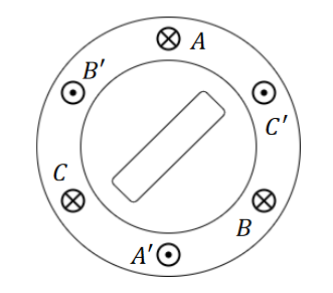
\includegraphics[width=0.8\linewidth]{Resumen_14} % Cambia "Resumen_14" a la ruta correcta de tu imagen
    \captionof{figure}{Generador síncrono trifásico}
\end{minipage}

\vspace{0.5cm} % Espacio opcional para separar la imagen del inicio del itemize

\begin{itemize}
  \item El rotor, que proporciona el campo, puede ser un imán permanente. Sin embargo, en la práctica se prefiere emplear un devanado excitado con corriente continua (devanado de campo), alimentado a través de anillos rozantes desde una fuente de CC, que puede ser una batería u otra máquina eléctrica operando como generador, la cual se denomina \textbf{Excitatriz}.
  \item El campo magnético rotatorio (CMR) es el campo magnético resultante de la interacción de las fuerzas magnetomotrices de los 3 enrollados del estator de una máquina sincrónica trifásica, cuando éstos son alimentados desde una fuente trifásica de voltaje de CA y se mueve a una velocidad de sincronismo $w_{s}$.
  \item Un motor síncrono en régimen permanente opera siempre a la misma velocidad cualquiera sea la carga en el eje.
  \item $\Delta$ Está relacionado con la carga del motor; mientras mayor carga, más grande será el valor de dicho ángulo.
  \item La velocidad mecanica del rotor $n_{m}$ es igual a la velocidad sincronica $n_{s}$ (\textit{Que es la velocidad con la que gira el CMR}) tenemos por otro lado que las variables \textbf{electricas} se relacionan con la velocidad sincronica $n_{s}$ mediante $n_{s} =\frac{120}{p}f$
\end{itemize}
\section*{Aspectos constructivos y modelo circuital}
\begin{itemize}
  \item El estator está compuesto por un paquete de láminas de acero, aisladas entre sí, con
  el propósito de reducir las pérdidas en el núcleo por corrientes parásitas
  \item Existen dos tipos de rotores con circuito de campo, siendo el rotor de polos salientes y el rotor cilindrico
\begin{figure}[H]
  \centering
  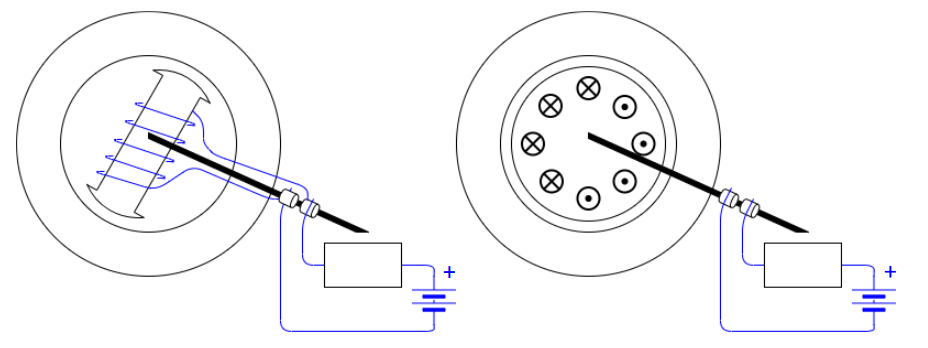
\includegraphics[width=0.4\textwidth]{Resumen_15}
  \caption{Rotor de polos salientes y rotor cilindrico}
\end{figure}
  \item Dado que se requiere suministrar una corriente CC al circuito de campo del rotor, existen dos posibles formas:
  \begin{itemize}
    \item Desde una fuente externa CC por medio de anillos rozantes y escobillas
    \item Desde una fuente de potencia de CC especial montada directamente en el eje del generador sincronismo
  \end{itemize} 
  \item Existen varios factores que ocasionan que E y V sean diferentes algunos de estos son:
  \begin{itemize}
    \item Reaccion de armadura
    \item Autoinductancia de las bobinas de la armadura
    \item Resistencia de las bobinas de armadura
    \item Efecto de la forma del rotor de polos salientes
  \end{itemize}
\end{itemize}
Si se considera que $x_{d} = x_{q} = x_{s}$, siendo la ultimma llamada reactancia sincronica, se tiene lo siguiente:
\begin{align}
  \text{Motor:} \quad \hat{V} &= j x_s \hat{I} + \hat{E} \\
  \text{Generador:} \quad \hat{E} &= j x_s \hat{I} + \hat{V}
\end{align}
\begin{figure}[H]
  \centering
  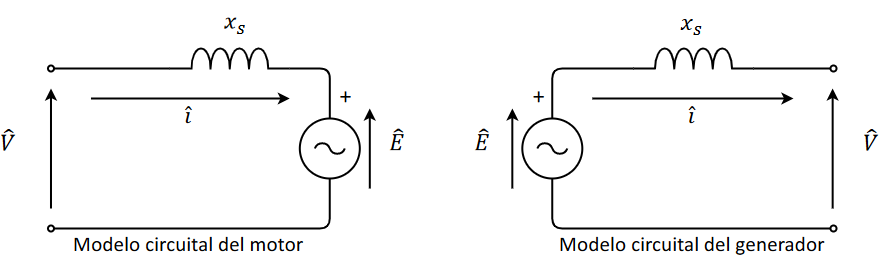
\includegraphics[width=0.8\textwidth]{Resumen_16}
  \caption{Modelo circuital de una maquina sincrona operando tanto como motor y generador, por lo general el termino resistivo suele ser despreciable, por lo que a terminos practicos solo se considerara $x_{s}$}
\end{figure}
Para determinar de manera experimental la reactancia sincronica de una maquina sincronica de rotor cilindrico se necesitan las curvas de excitacion y cortocircuito, las cuales son:
\begin{figure}[H]
  \begin{center}
    \subfigure[La \textbf{curva de excitación o de saturación en vacío} muestra la relación entre la tensión en bornes de la máquina (en vacío) y la corriente de excitación \( i_r \) del rotor. En condiciones de vacío (sin corriente de estator), la tensión en bornes es igual a la tensión interna, es decir, \(\hat{E} = \hat{V}\) y esta relación \(E = f(i_r)\) tiene una forma similar a la curva \( B-H \) del núcleo, ya que la fem \( E \) es proporcional al flujo magnético.]{
        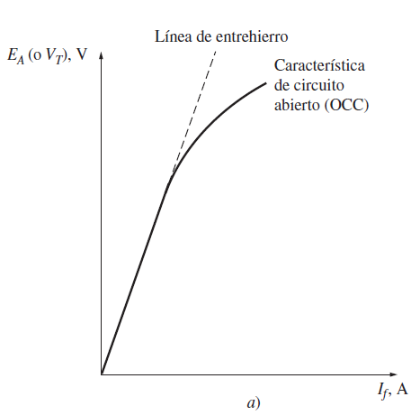
\includegraphics[width=0.35\textwidth]{Resumen_17}
        \label{Imagen-Madrid}}
    \hspace{0.5cm} % Espacio horizontal entre las imágenes
    \subfigure[Se obtiene la curva de cortocircuito cortocircuitando los terminales del estator y aumentando la corriente de campo, asegurándose de no exceder el valor nominal de la corriente de armadura. En esta condición, la corriente de cortocircuito se retrasa casi 90° respecto a la fem debido a la predominancia de la reactancia sobre la resistencia en la impedancia sincrónica. La relación entre la fem y la corriente de excitación genera una característica lineal de cortocircuito que permite calcular la impedancia sincrónica en condiciones de saturación y sin saturación.]{
        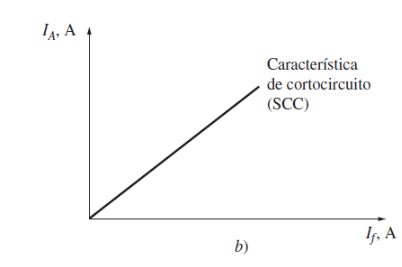
\includegraphics[width=0.45\textwidth]{Resumen_18}
        \label{Imagen-Londres}}
    \caption{Curvas de excitación y cortocircuito.}
    \label{Figura-Curvas}
  \end{center}
\end{figure}
\begin{minipage}{0.6\textwidth} % Parte izquierda con el texto y ecuaciones
  En la figura, \( \overline{AB} \) representa el voltaje en vacío con la corriente de excitación \( i_{r1} \), y \( \overline{AD} \) es la corriente de armadura obtenida con \( i_{r1} \) en cortocircuito. La impedancia sincrónica saturada queda dada por:
  \[
  z_s = \frac{\overline{AB} \, [V]}{\overline{AD} \, [A]}
  \]

  La impedancia sincrónica no saturada se expresa como:
  \[
  z_s = \frac{\overline{AC} \, [V]}{\overline{AD} \, [A]}
  \]
\end{minipage}%
\hfill
\begin{minipage}{0.3\textwidth} % Parte derecha con la imagen
  \centering
  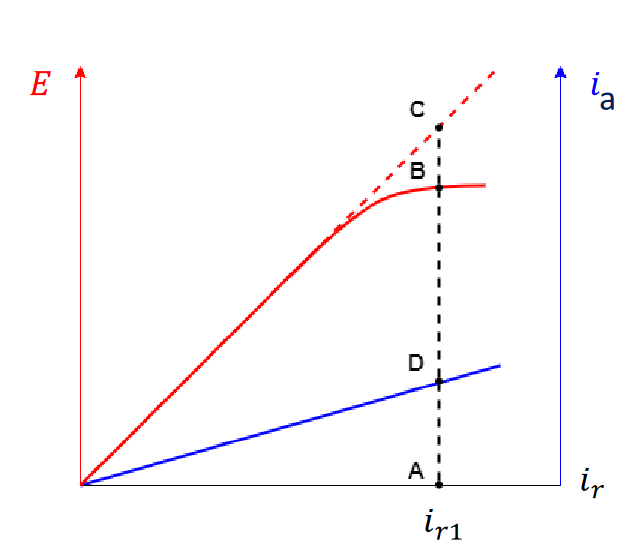
\includegraphics[width=1\linewidth]{Resumen_19} % Ajusta la ruta de la imagen si es necesario
  \captionof{figure}{Curva de cortocircuito y excitación de una máquina síncrona}
\end{minipage}
\section*{Analisis en estado estacionario}
Las potencias  monofasicas tanto en generador como en motor en los terminales de la maquina cuando se desprecia $r_{s}$ y ademas se considera que $x_{d}= x_{q} = x_{s}$ seran:
\begin{align}
  P &= \frac{VE}{x_{s}}sin(\delta)\\
  Q &= \frac{V}{x_{s}}(Ecos(\delta) -V)\\
  T &= \frac{P}{w_{s}} = \frac{P}{4\pi f}3P
\end{align}
\begin{figure}[H]
  \begin{center}
    \subfigure[Diagramas fasoriales ]{
        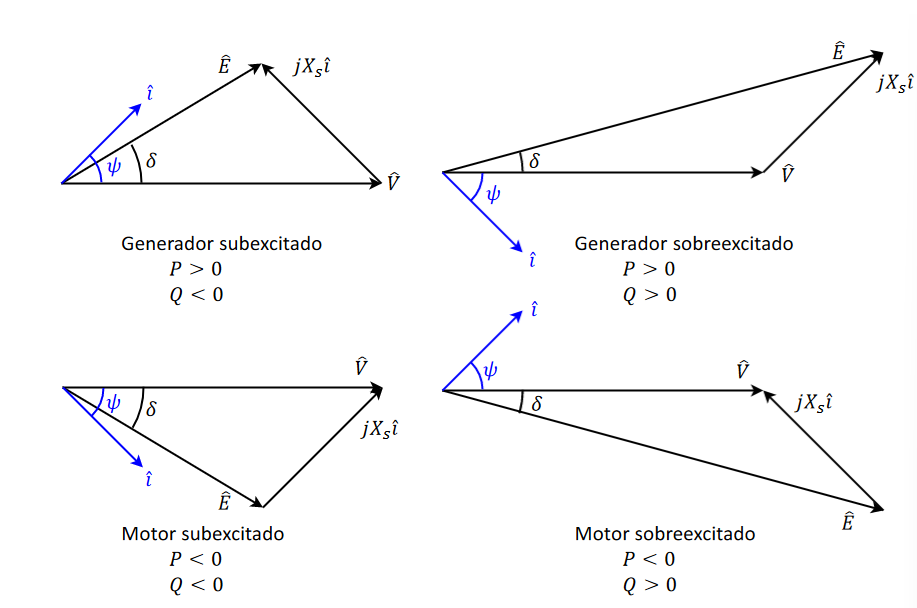
\includegraphics[width=0.4\textwidth]{Resumen_20}
        \label{Imagen-Madrid}}
    \hspace{0.5cm} % Espacio horizontal entre las imágenes
    \subfigure[Diagramas fasoriales en el plano rectangualr]{
        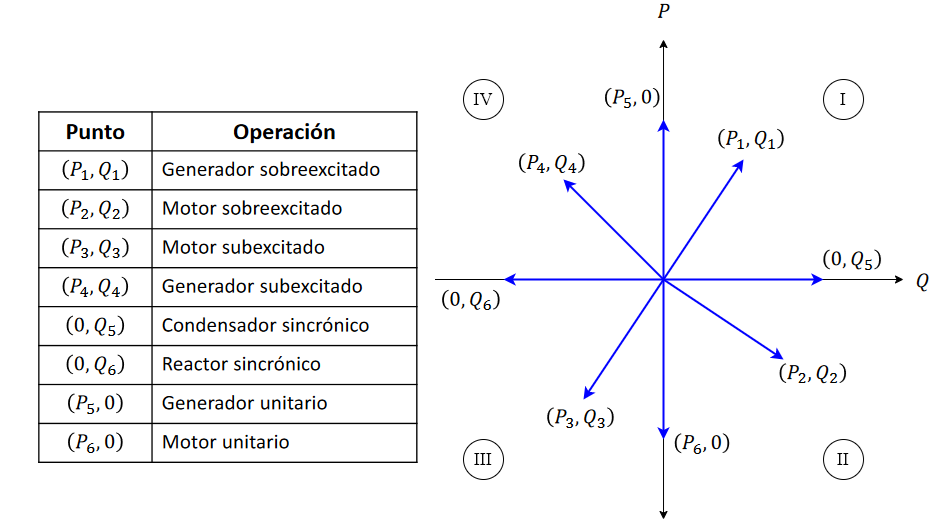
\includegraphics[width=0.45\textwidth]{Resumen_21}
        \label{Imagen-Londres}}
    \label{Figura-Curvas}
  \end{center}
\end{figure}
Un generador síncrono puede verse como un sistema con dos variables de entrada o de control (Torque mecánico \( T_m \) y la corriente de excitación \( i_{r_s} \)) y cuatro variables de salida (las potencias activa \( P \) y reactiva \( Q \), la tensión en bornes \( V \) y la frecuencia eléctrica \( f \)). Se pueden estudiar dos casos extremos de operación:

\begin{itemize}
    \item En un \textbf{sistema de barra infinita} (es decir, un sistema muy grande comparado con el generador), la frecuencia y la tensión se mantienen constantes, sin importar el torque o la excitación aplicada a la máquina. Esto simplifica el control al desacoplar las variables de entrada y salida, ya que solo las potencias activa \( P \) y reactiva \( Q \) se ven afectadas. Normalmente, la potencia activa \( P \) se ajusta mediante el torque mecánico de entrada \( T_m \) a través del ángulo de carga \( \delta \), mientras que la potencia reactiva \( Q \) se controla variando la excitación \( i_r \) del generador.

    \item En el \textbf{modo de operación en isla}, el generador, donde alimenta únicamente una impedancia, no se observan variables constantes ni desacoples. Un aumento en el torque mecánico \( T_m \) provoca una aceleración del rotor, lo cual incrementa la frecuencia eléctrica y la tensión en bornes \( V \). A su vez, un incremento en la corriente de excitación eleva \( E \) y \( V \). En este modo de operación, cualquier aumento en \( V \) (y/o \( f \)) resultará en un incremento de las potencias activa \( P \) y reactiva \( Q \).
\end{itemize}

Las cartas de operación se emplean para determinar gráficamente las condiciones de operación de un generador conectado a un sistema eléctrico comparativamente grande. Son curvas de igual excitación, calculadas para una frecuencia y una tensión constantes y dibujadas en un sistema de ejes cartesianos P-Q, en el cual se incluyen también los límites de la zona de operación:

\begin{itemize}
    \item \textbf{Máxima y mínima potencia activa}: En un generador, \( P \geq 0 \), donde el límite inferior es determinado por razones de manejo del fuego en generadores térmicos de rotor cilíndrico, que fijan \( P_{\text{min}} \) en torno al 30% de la potencia nominal. La turbina puede imponer un límite máximo \( P_{\text{max}} \) en la potencia activa debido a sus propias restricciones. Aunque en una central bien planificada el generador debiera ajustarse a la potencia de la turbina, en algunos casos el límite \( P_{\text{max}} \) puede estar fuera del diagrama.

    \item \textbf{Máxima corriente de armadura}: En las máquinas reales, la corriente de armadura tiene un valor máximo impuesto por el calentamiento del estator y la vida útil del aislamiento. Este límite establece una circunferencia con centro en el origen y radio \( V_{\text{max}} \). Por razones económicas, se opera con una combinación de \( P \) y \( Q \), por lo que este límite es ligeramente superior al de la máxima potencia activa, es decir, \( V_{\text{max}} \geq P_{\text{max}} \). En la intersección de ambos límites se alcanza el factor de potencia nominal. Este límite puede sobrepasarse brevemente ya que se relaciona con el calentamiento acumulado.

    \item \textbf{Máxima y mínima corriente de excitación}: Dado que existe un valor máximo para la corriente de excitación, impuesto por el calentamiento del rotor o las características de la excitatriz, se genera un límite para la operación del generador, representado por una circunferencia de centro \( V_{\text{nom}} \) y radio \( \frac{V_{\text{max}}}{X_s} \). Este límite es generalmente inferior al de la corriente de armadura solo para cargas inductivas pequeñas. En general, se estima una excitación mínima \( E_{\text{min}} \), generando así un límite de operación con centro \( \left( \frac{V_{\text{nom}}^2}{X_s}, 0 \right) \) y radio \( \frac{V_{\text{nom}} \cdot E_{\text{min}}}{X_s} \). Esto limita la potencia reactiva absorbida por el generador.

    \item \textbf{Límite de estabilidad permanente}: Existe una limitación de operación en una máquina síncrona impuesta por la inestabilidad que ocurre al alcanzar un ángulo de carga \( \delta = 90^\circ \) en máquinas de rotor cilíndrico. Este límite teórico se representa como una recta paralela al eje \( P \), que pasa por el punto \( \left( -\frac{V^2}{X_s}, 0 \right) \), donde la potencia reactiva \( Q \) es negativa. Debido a que trabajar en este límite es poco aconsejable y difícil de controlar, se define un \textbf{límite práctico de estabilidad}, generalmente basado en experiencias de operación. Este límite práctico se representa como una recta que parte del punto \( \left( -\frac{V^2}{X_s}, 0 \right) \) y forma un ángulo de 70° con respecto al eje de la potencia reactiva \( Q \).
\end{itemize}

\begin{figure}[H]
  \centering
  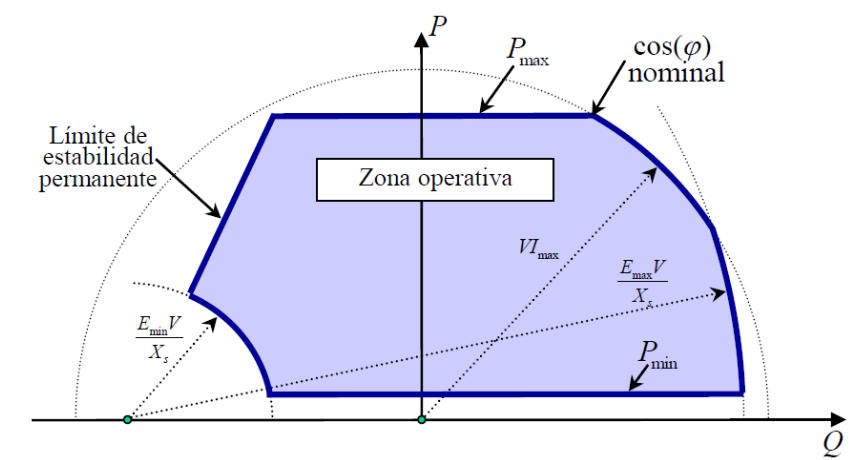
\includegraphics[width=0.6\textwidth]{Resumen_22}
  \caption{Ejemplo de carta de operación de un generador síncrono}
\end{figure}
%------------------------------
\newpage
\hrule
\section*{Ejemplos: Preguntas de contenido Maquinas Sincronas}
\begin{questions}
  \question \textbf{(Control 2 Primavera 2023)}¿Cuál es la desventaja del uso de escobillas para la alimentación del campo eléctrico de la máquina
  síncrona? Mencione una alternativa de alimentación del campo eléctrico que no requiera su uso.
  \begin{solution}
    Las escobillas sufren de desgaste, por lo que las máquinas síncronas en las que el campos es alimentado mediante ellas, deben ser sometidas a mayor mantención.\\\\
    Una alternativa de alimentación del campo eléctrico es el uso de un circuito excitador sin escobillas en el que se instala un bobinado menor en la armadura el cual induce una excitación trifásica en el rotor, la cual es rectificada para alimentar el campo
  \end{solution}
  \question \textbf{(Control 2 Primavera 2023)} Explique en qué consiste el campo magnético rotatorio de la máquina síncrona y cómo se genera. Utilice ecuaciones
  \begin{solution}
    El campo magnético rotatorio (CMR) es el campo magnético resultante de la interacción de las fuerzas magnetomotrices de los 3 enrollados del estator cuando estos son alimentados desde una fuente trifásica de voltaje AC. Así se tiene que la fmm resultante es de magnitud constante y gira en el espacio a la velocidad de sincronismo.

Así se obtienen las siguientes ecuaciones para el CMR:

\begin{itemize}
    \item[a)] \textbf{Corriente estator}
    \begin{align*}
        i_a &= I_m \cdot \cos(w_s \cdot t) \\
        i_b &= I_m \cdot \cos(w_s \cdot t - 120^\circ) \\
        i_c &= I_m \cdot \cos(w_s \cdot t - 240^\circ)
    \end{align*}

    \item[b)] \textbf{FMM resultante}
    \begin{align*}
        F_a &= N \cdot I_m \cdot \cos(w_s \cdot t) \\
        F_b &= N \cdot I_m \cdot \cos(w_s \cdot t - 120^\circ) \\
        F_c &= N \cdot I_m \cdot \cos(w_s \cdot t - 240^\circ)
    \end{align*}

    \item[c)] \textbf{Proyección y z}
    \begin{align*}
        F_y &= \frac{3}{2} \cdot N \cdot I_m \cdot \cos(w_s \cdot t) = \frac{3}{2} \cdot N \cdot I_m \cdot \cos(w_s \cdot t) \\
        F_z &= \frac{3}{2} \cdot N \cdot I_m \cdot \sin(w_s \cdot t)
    \end{align*}
\end{itemize}
  \end{solution}
  \question \textbf{(Control 2 Otoño 2024)} La acción conjunta de los generadores síncronos en las centrales de generación eléctrica es la que princi-
  palmente fija la frecuencia eléctrica y tensión de la red, incluso en los puntos de consumo.
  \begin{solution}
    Verdadero. En general en los SEP hay varios generadores operando en paralelo para suministrar la demanda de energía requerida por las cargas, siendo la frecuencia y la magnitud de la tensión en los SEP un resultado de la acción conjunta de todas las máquinas síncronas que se encuentran girando.
  \end{solution}
  \question \textbf{(Control 2 Otoño 2024)} En la carta de operación de un generador sincrónico, la limitación de potencia aparente máxima viene
  dada por las capacidades de corriente y tensión de los enrollados de estato
  \begin{solution}
    Verdadero. Aunque se asume la tensión en bornes y frecuencia constante para graficar la carta de operación. Existe una limitación en la carta de operación superior a la potencia máxima activa dada $P_{max} \leq V i_{max}$, la cual corresponde al radio de una circunferencia
  \end{solution}

\end{questions}
\end{document}